\chapter{Proposta}\label{chp:PROPOSTA}

% falar sobre o capitulo

Este capítulo é responsável por apresentar o sistema proposto, sua motivação e modelagem.
A seção \ref{sec:motivacao} identificará a problemática acerca da avaliação do Ensino Superior sendo realizada de forma genérica, sugerindo a necessidade de uma avaliação interna e automatizada. Já na seção \ref{sec:trab_relacionados}, serão identificados sistemas que tenham a proposta semelhante com a deste projeto, bem como universidades que aplicam suas próprias avaliações. Enquanto a seção \ref{sec:proposta} apresentará a modelagem da solução proposta.

\section{Motivação}
\label{sec:motivacao}

% Intro
% SINAES

No Brasil, por meio da \citeonline{lei10861} as instituições de ensino superior devem estar de acordo com as normas do Sistema Nacional de Avaliação da Educação Superior (SINAES)
cujo objetivo é contribuir para a melhoria contínua dos cursos e instituições avaliando 
os aspectos relacionados ao ensino, pesquisa, extensão, do corpo docente, da gestão institucional, bem como a responsabilidade social e infraestrutura.

% Problema: SINAES mt abrangente

A avaliação institucional desempenha um papel crucial na melhoria contínua da qualidade educacional
e é uma tarefa complexa que demanda a consideração de vários fatores. Embora o SINAES seja fundamental para esse processo no Brasil, sua metodologia geral de avaliação é aplicada a todas as áreas do conhecimento, o que pode não levar em conta especificidades de determinadas áreas.

% Problema: 

Os discentes são os principais protagonistas desse processo, sendo diretamente impactados pelas disciplinas cursadas e pelos professores que as ministraram. Ao avaliar esses elementos, os estudantes podem manifestar suas opiniões, pontuar se o conteúdo está alinhado às expectativas e se é relevante para sua formação. Além disso, uma avaliação do professor possibilita uma análise aprofundada do seu desempenho, levando em conta didática, comunicação e capacidade de estimular o interesse do aluno.

% Mas pq um sistema web? %
% -> Privacidade do aluno ao dar o feedback
% -> Agilidade e eficiencia na coleta e análise dos dados
% -> Acompanhamento em tempo real 
% -> Fácil acesso

% Introdução da Solução: Sistema próprio da universidade de avaliação

Para que a instituição esteja preparada para enfrentar desafios, é necessário que seus membros tenham ciência de sua realidade, virtudes, capacidades e limitações.
%Nelson de Abreu Júnio[2] (2009)
De acordo com \citeonline{junior_2009}, os processos avaliativos precisam envolver o maior número de participantes, tanto na construção de seu projeto quanto na análise e no uso dos resultados, contribuindo para o desenvolvimento humano.

% Solução: Sistema próprio da universidade de avaliação

Não restam dúvidas quanto à importância das universidades no desenvolvimento do país, sendo fundamental uma administração adequada e alinhada às suas necessidades. Nesse sentido, e como afirmaram \citeonline{selfEvaluation2012}, as instituições devem se esforçar para estabelecer um sistema interno de garantia da qualidade que forneça uma base genuína para a tomada de decisões de gestão. 
% A melhoria dos sistemas de ensino superior em países em desenvolvimento requer uma autoavaliação. Nesse contexto, e de acordo com \citeonline{betts1992}, há a necessidade de desenvolver uma capacidade aumentada de autoreflexão, autodireção e autorrenovação no ambiente de ensino superior. Tornando-se fundamental que a 

Atualmente, estamos imersos em um contexto em que a tecnologia se tornou onipresente, desempenhando um papel indispensável em nossas vidas e influenciando para além de nossas atividades cotidianas. Considerando essa realidade, torna-se essencial que essa avaliação institucional realizada pelas próprias instituições de ensino seja realizada de forma automatizada. 

A utilização de sistemas e plataformas digitais permite que as universidades coletem, processem e analisem os dados de maneira precisa e eficiente, respeitando a privacidade dos alunos. Além disso, a automação desse processo reduz o tempo necessário para a obtenção dos resultados, permitindo que a instituição colete os dados quantitativos e qualitativos de maneira abrangente, envolvendo um maior número de estudantes.

% TODO: Talvez seja interessante amarrar esse texto que vocês fizeram com o objetivo do seu trabalho. Algo simplório.

%\cite{braida2015transforming}
%\citeonline{braida2015transforming}

% justificar melhor o trabalho

\section{Trabalhos Relacionados}
\label{sec:trab_relacionados}
% Neste tópico serão apresentados alguns sistemas de avaliação aplicados por universidades e trabalhos acerca da avaliação institucional no ensino superior.

De uma maneira mais geral, temos o 
\textit{Rate my Professors}\footnote{\url{https://www.ratemyprofessors.com/}}, 
um dos \textit{websites} mais populares nos Estados Unidos para que os estudantes possam pesquisar e avaliar professores e universidades. Esse recurso foi desenvolvido com o intuito de auxiliar outros estudantes universitários em suas decisões ao escolherem suas aulas e professores, com o objetivo de que as opiniões dos discentes poderiam beneficiar futuros estudantes, promovendo assim uma seleção mais transparente e embasada. O \textit{site} proporciona um \textit{feedback} dos usuários sobre a metodologia de ensino dos professores e suas disciplinas, incluindo uma avaliação das instalações dos campi universitários. Vale ressaltar que apenas os alunos que tenham frequentado uma aula do professor em questão ou que estejam atualmente matriculados nessa disciplina são autorizados a compartilhar suas avaliações, sendo limitados a um único comentário.

% que foi criado com a motivação de ajudar outros estudantes universitários a tomar decisões informadas ao escolher suas aulas e professores, acreditando que as opiniões dos alunos poderiam ajudar futuros alunos, tornando a seleção de aulas e professores mais transparente e informada.

Já no contexto brasileiro, a Universidade Federal Fluminense (UFF) possui a Comissão Própria de Avaliação Institucional da UFF (CPA/UFF),
responsável pela formulação do instrumento de avaliação da Universidade, conhecido como Sistema de Avaliação Institucional (SAI)\footnote{\url{https://app.uff.br/sai}}.
O SAI foi desenvolvido com o propósito de coletar a perspectiva dos alunos e professores sobre os cursos de graduação,
mediante a avaliação do desempenho efetivo nas disciplinas e da disponibilidade de infraestrutura para o seu funcionamento.
Os resultados obtidos por meio dessa avaliação são analisados pela CPA/UFF, pelas Unidades Acadêmicas, pelos Departamentos de Ensino e pelas Coordenações de Curso,
e servem como base para a reflexão acerca da qualidade do trabalho acadêmico realizado na UFF, gerando informações relevantes e necessárias para a reformulação dos Projetos Pedagógicos dos Cursos.

Falar sobre universidades que aplicam avaliações internas:
 Exemplo: 
 Universidad de Buenos Aires (UBA)
 Universidade de São Paulo (USP) = Avaliação Institucional da USP
     Universidade Federal FLuminense (UFF) = Avaliação Institucional da UFF

\section{Proposta}
\label{sec:proposta}

% intro + o que é o projeto 
Conforme supracitado, a qualidade do ensino é um elemento crucial para o desenvolvimento dos estudantes e para o aprimoramento das instituições de ensino. Visando promover uma educação cada vez mais eficiente e participativa, este trabalho propõe o desenvolvimento de um sistema \textit{web} de avaliação de disciplinas para o curso de Ciência da Computação da Universidade Federal Rural do Rio de Janeiro - Instituto Multidisciplinar (UFRRJ/IM), com o objetivo de oferecer \textit{feedback} periódico e valioso para o aperfeiçoamento contínuo do processo educacional e viabilizando uma relação de transparência e qualidade no ambiente acadêmico.

%objetivos 

O projeto tem como objetivo analisar o desempenho das disciplinas ofertadas no período letivo decorrido, coletando informações sobre a eficácia, organização e relevância. Os alunos serão estimulados a avaliar aspectos como o conteúdo ministrado, a metodologia aplicada, avaliações e recursos didáticos afim de identificar pontos fortes e fracos de cada uma bem como examinar a atuação dos professores, buscando avaliar o desempenhos dos professores no processo de ensino-aprendizagem, serão considerados critérios como o domínio sobre a matéria, didática, clareza sobre a ementa, comunicação compreensiva, disponibilidade e capacidade de manter os alunos motivados.

% metodologia

Para a realização da avaliação, foi desenvolvida uma plataforma \textit{online} que permite aos alunos expressar suas opiniões de forma segura e anônima e aos professores e gestores acompanhar as métricas através de uma análise das avaliações. Os resultados serão apresentados de maneira estruturada e compreensível em um \textit{dashboard}, que permitirá que os professores acompanhem suas próprias avaliações e que os coordenadores tenham acesso às avaliações do corpo docente sob o qual é responsável.

Foram elaborados questionários estruturados que abordam os diferentes aspectos relacionados às disciplinas cursadas e aos professores que as ministraram. Os questionários são compostos com questões de escalas de avaliação de 1 a 5, sendo 1 muito ruim e 5 muito bom, e campos de comentários abertos tanto de sugestões quanto para a identificação de pontos positivos e negativos. É importante ressaltar a confidencialidade das respostas dos estudantes. O sistema garantirá o anonimato dos discentes, encorajando a participação franca e honesta permitindo que os estudantes sintam-se a vontade para expressar suas opiniões de forma livre e sem receio de represálias.

%A plataforma também disponibilizará uma análise das avaliações. Os resultados serão apresentados de maneira estruturada e compreensível em um \textit{dashboard}, que permitirá que os professores acompanhem suas próprias avaliações e que os coordenadores tenham acesso às avaliações do corpo docente sob o qual é responsável.

Os professores terão acesso a uma visão geral das avaliações recebidas em suas disciplinas. 
%Para os professores, o \textit{dashboard} irá fornecer uma visão geral das avaliações recebidas em suas disciplinas. 
Eles conseguirão visualizar os resultados de forma consolidada, como médias e comentários feitos pelos discentes, podendo compreender com mais clareza o \textit{feedback} recebido e identificar áreas de destaque e oportunidade de melhorias, além de admitir uma análise com avaliações anteriores e com as médias da instituição. Já para os coordenadores será disponibilizada uma análise mais abrangente, tendo acesso às avaliações dos professores sob sua responsabilidade, permitindo uma análise comparativa e um acompanhamento mais efetivo do desempenho docente. 

Essa iniciativa busca fortalecer o diálogo entre alunos e instituição, disponibilizando avaliações de disciplinas e professores, bem como sua análise, para a comunidade acadêmica. O objetivo é aprimorar o gerenciamento das informações, promover transparência, autoaperfeiçoamento docente e demonstrar o compromisso da universidade em atender as necessidades e expectativas dos estudantes com base em dados.% A seguir serão apresentados informações mais detalhadas sobre o planejamento e desenvolvimento do Sistema de Avaliação de Disciplinas.


%% Falar um pouco + a fundo das métricas usadas (?)
% escala de 5(?) estrelas sendo 1(mt ruim) e 5(mt bom) ok
% Exemplo do questionároi (?)






\begin{comment}
O intuito desse trabalho é desenvolver um sistema web de avaliação de disciplinas para o curso de Ciência da Computação da Universidade Federal Rural do Rio de Janeiro - Instituto Multidisciplinar (UFRRJ/IM), com o objetivo de auxiliar o departamento do curso a tomar decisões que visem melhorar o ensino e aprendizado dos alunos.

O sistema permite que os aluno acessem um questionário de avaliação para cada disciplina em que ele estava matriculado. Esse questionário conta com perguntas que podem medir a qualidade da didática do professor, a ementa da disciplina, as avaliações, entre outros.

O sistema conta com uma tela de cadastro que pode ser usada tanto por alunos e professores da universidade e uma tela de login. Caso o usuário logado seja um aluno, ele poderá visualizar uma lista das disciplinas em que ele estava matriculado. O aluno pode avaliar cada disciplina dessa lista somente uma vez. Caso o usuário logado seja um professor, ele terá acesso a uma lista de disciplinas lecionadas por ele. Cada disciplina contará com um relatório com a média de avaliações recebidas. Caso o usuário seja um administrador, ele poderá acessar todas as disciplinas do curso de Ciência da Computação da UFRRJ, e visualizar o relatório de avaliações para cada uma delas.

Administradores do sistema poderão cadastrar períodos e disciplinas, e associar os professores a suas respectivas disciplinas. 
\end{comment}

\subsection{Atores}
Um ator é uma entidade externa que interage com o sistema e desempenha um papel específico dentro do contexto do sistema em análise. Ao identificar os atores, é possível determinar quais são as suas responsabilidades e como eles se relacionam com as funcionalidades do sistema. Essas informações são utilizadas para modelar os casos de uso e requisitos do sistema.

Com base na proposta apresentada anteriormente, é possível identificar os seguintes atores:

\begin{alineas}
  \item \textbf{Aluno} Representa os alunos do curso de Ciência da Computação. Eles podem visualizar a lista de disciplinas em que estão matriculados e avaliá-las uma vez, após o encerramento do período letivo.
  \item \textbf{Professor} Representa os professores responsáveis pelas disciplinas do curso. Eles podem visualizar as disciplinas que lecionam e acompanhar um relatório com as avaliações recebidas para cada uma delas.
  \item \textbf{Coordenador} Representa o(s) coordenador(es) do curso. Eles têm a responsabilidade de cadastrar disciplinas, associar os professores às disciplinas ministradas por eles, e, principalmente, visualizar relatórios com as avaliações de cada disciplina. Esses relatórios são fundamentais para análise de resultados e tomadas de decisões estratégicas para melhorar a qualidade do curso.
\end{alineas}

Esses atores desempenham papéis distintos no sistema de avaliação de disciplinas, e cada um contribui de uma maneira para o funcionamento do sistema.

\subsection{Questionário}

%Falar sobre o questionário.
O questionário de avaliação de disciplina e do docente foi elaborado para capturar informações pertinentes acerca da experiência dos estudantes em relação à disciplina cursada, permitindo a identificação de pontos fortes e áreas passíveis de aprimoramento.

Optamos pela utilização de um conjunto de questões pré definidas visando a padronização das respostas. Além disso, para assegurar que os objetivos da organização sejam atendidos de forma adequada. Outra vantagem é a comparabilidade dos resultados, sendo possível comparar diferentes disciplinas, professores e períodos letivos.


Questões:
\begin{alineas}
\item Com base no período corrente quanto você avalia que foi a didática do(a) professor(a)?
\item Com base no período corrente quanto você avalia que foi a pontualidade do(a) professor(a)?
\item Com base no período corrente quanto você avalia que foi a assiduidade do(a) professor(a)?
\item Com base no período corrente quanto você avalia que o(a) professor(a) cumpriu a ementa da disciplina?
\item Você conseguiu perceber, com base nas aulas do(a) professor(a) a interdiciplinalidade do conteúdo dado?
\item Com base no período corrente quanto você avalia que foram as avaliações (trabalhos, provas, teste, etc) do(a) professor(a)?
\item Com base no período corrente quanto você avalia a forma de cobrar o conteúdo dado pelo(a) professor(a)?
\item Faça uma breve descrição dos pontos positivos percebidos nessa disciplina:
\item Faça uma breve descrição dos pontos negativos percebidos nessa disciplina:
\end{alineas}


\subsection{Regras de Negócio}
As regras de negócio definem diretrizes e restrições de uma aplicação. Elas são essenciais para que haja clareza do que deve ser feito ao desenvolver um sistema, atendendo às necessidades e requisitos do negócio. Algumas das regras de negócio aplicadas ao sistema de avaliação de disciplinas são:

% escrever mais regras de negócio

\begin{alineas}
  \item \textbf{RN1 - Restrição de matrícula} O Aluno só pode avaliar em que ele esteja matriculado: Não é permitido avaliar disciplinas não cursadas.
  \item \textbf{RN2 - Restrição de avaliação única} O Aluno só pode avaliar uma disciplina uma única vez: Cada disciplina pode ser avaliada somente uma vez por cada aluno.
  \item \textbf{RN3 - Restrição de anonimato} O Aluno não pode ser identificado na avaliação: A avaliação deverá ser anônima.
  \item \textbf{RN4 - Restrição de acesso aos relatórios} O Professor pode visualizar somente os relatórios de suas disciplinas: Não é permitido acessar relatórios de outros professores.
  \item \textbf{RN5 - Acesso do Coordenador aos relatórios} O Coordenador pode ver relatórios de todas as disciplinas: O Coordenador deve ter uma visão geral com todos os relatórios de avaliações das disciplinas do curso.
  \item \textbf{RN6 - Cadastro de disciplinas} O Coordenador pode cadastrar disciplinas: Somente o Coordenador pode realizar cadastros de disciplinas e associar professores a elas.
\end{alineas}

Esses exemplos destacam algumas das regras de negócio cruciais para o funcionamento do sistema de avaliação de disciplinas. Ao seguir essas regras, é possível desenvolver uma aplicação segura, eficiente e que respeite a privacidade dos dados dos usuários.

\subsection{Requisitos do Sistema}
Os requisitos do sistema são descrições sobre o que o sistema deve ser capaz de fazer para atender às regras de negócios. Esses requisitos são divididos em requisitos funcionais e não funcionais. 

Os requisitos funcionais especificam funcionalidades que o sistema deve ter para atender às necessidades do usuário final. Já os requisitos não funcionais especificam as restrições e limitações da aplicação.

Alguns requisitos funcionais do sistema de avaliação de disciplina são:

% escrever mais requisitos

\begin{alineas}
    \item \textbf{RF1 - Cadastrar disciplina} O Coordenador poderá cadastrar disciplinas informando nome, turno, professor e período letivo.
    \item \textbf{RF2 - Editar disciplina} O Coordenador poderá editar o nome, turno, professor e período letivo de uma disciplina.
    \item \textbf{RF3 - Excluir disciplina} O Coordenador poderá excluir uma disciplina.
    \item \textbf{RF4 - Listar disciplinas} O usuário poderá visualizar uma lista de disciplinas.
    \item \textbf{RF5 - Cadastrar período} O Coordenador poderá incluir um período letivo informando o ano e o semestre.
    \item \textbf{RF6 - Editar período} O Coordenador poderá editar o ano de um período letivo cadastrado no sistema.
    \item \textbf{RF7 - Excluir período} O Coordenador poderá excluir um período letivo.
    \item \textbf{RF8 - Visualizar relatórios} O Coordenador e o Professor poderão visualizar relatórios de avaliações.
\end{alineas}

Ao satisfazer todos os requisitos do sistema, podemos garantir que o software é confiável e funcional. 

\subsection{Casos de Uso}
Os casos de uso representam interações entre os atores e o sistema. Eles documentam as principais funcionalidades do sistema do ponto de vista do usuário final. 

% escrever corretamente os casos de uso

Alguns casos de uso do sistema de avaliação de disciplina são:

\begin{alineas}
    \item \textbf{Efetuar login}
        \begin{alineas}
            \item \textbf{Ator} Aluno, Professor ou Coordenador.
            \item \textbf{Descrição} Autenticação de usuários cadastrados no sistema, permitindo a realização de operações restritas à cada perfil.
        \end{alineas}
    \item \textbf{Visualizar disciplinas}
        \begin{alineas}
            \item \textbf{Ator} Aluno, Professor ou Coordenador.
            \item \textbf{Descrição} Visualização de informações das disciplinas: nome, turno, período letivo e professor.
        \end{alineas}
    \item \textbf{Avaliar disciplina}
        \begin{alineas}
            \item \textbf{Ator} Aluno.
            \item \textbf{Descrição} Avaliação da disciplina cursada no período letivo atual.
        \end{alineas}
    \item \textbf{Cadastrar disciplina}
        \begin{alineas}
            \item \textbf{Ator} Coordenador.
            \item \textbf{Descrição} Cadastro de uma disciplina no sistema informando nome, período letivo, turno e professor.
        \end{alineas}
    \item \textbf{Cadastrar período}
        \begin{alineas}
            \item \textbf{Ator} Coordenador.
            \item \textbf{Descrição} Cadastro de período letivo no sistema informando ano.
        \end{alineas}
    \item \textbf{Visualizar relatórios}
        \begin{alineas}
            \item \textbf{Ator} Coordenador ou Professor.
            \item \textbf{Descrição} Visualização de relatórios das avaliações feitas pelos alunos da disciplina.
        \end{alineas}
\end{alineas}

Os casos de uso listados exemplificam algumas das interações e funcionalidades mais importantes da aplicação.

\subsection{Diagrama de Entidade-Relacionamento}

O diagrama de entidade-relacionamento é usado para representar as entidades, seus atributos e seus relacionamentos, auxiliando na criação do banco de dados e servindo como base para o desenvolvimento do sistema. Assim, é possível analisar a estrutura da aplicação e identificar os relacionamentos entre as entidades.

Na figura \ref{fig:fig_diagrama_er} podemos observar a representação gráfica do diagrama ER do sistema de avaliação de disciplinas. Nesse diagrama, identificamos que a aplicação possui entidades como Usuário, onde serão armazenados os usuários e seus respectivos perfis (Aluno, Professor ou Coordenador), Disciplina, Avaliação, Período e a tabela intermediária DisciplinaAluno. 

\begin{figure}[h]
  \centering
  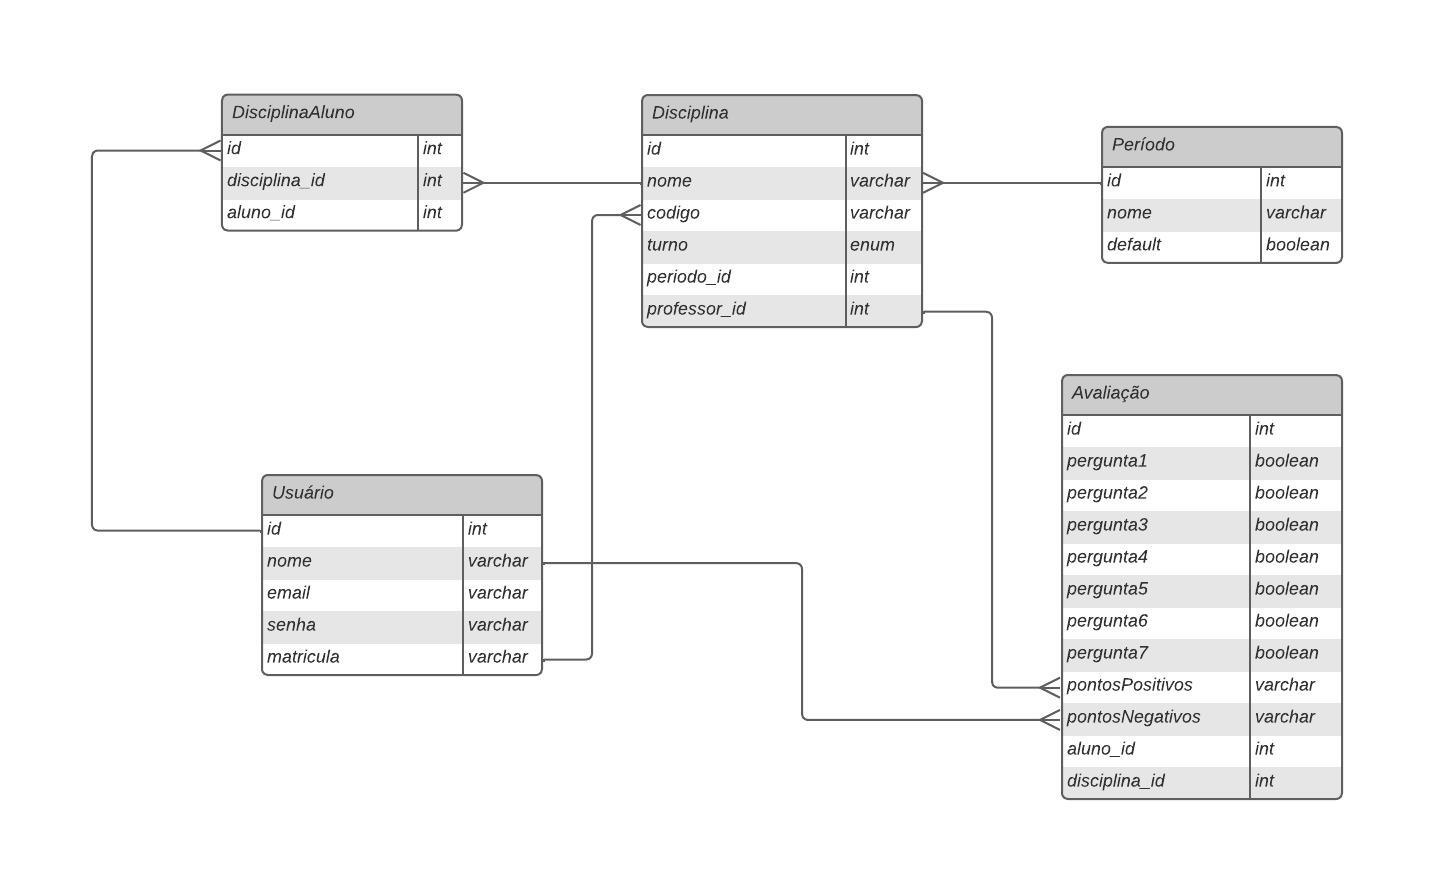
\includegraphics[width=1\textwidth]{imagens/diagrama-er-sistema-avaliacao-disciplina.jpeg}
  \caption{Diagrama ER da aplicação proposta}
  \label{fig:fig_diagrama_er}
  %\legend{Fonte: o autor.}
\end{figure}


% Explicar melhor tomadas de decisao na entidas
% Materias dividas em eriodos para saber onde
% Por que perguntas fixas
% (Falar mais do questionário de forma tecnica)
%
%
%



%%%%%%%%%%%%%%%%%%%%%%%%%%%%%%%%%%%%%%%%%%%%%%%%%%%%%%%%%%%%%%%%%%%%%
% [1] - Cad. Cedes, Campinas vol. 29, n. 78, p. 257-269, maio/ago. 2009 257 Disponível em <http://www.cedes.unicamp.br>
% [2] - 
% - Importâncida da avaliação institucional no que diz respeito de detectar demandas/melhorias/pontos fracos
% - SINAES como medidor de qualidade de ensino superior
% - Avaliação interna abrange situações/necessidades mais específicas
% - 
%

% Esse capítulo será responsável por explicar como será a sua solução.
% Ele deverá explicar o problema em que a sua solução irá resolver.
% Nele irá conter COMO deverá ser a sua solução, ou seja, neste momento você não está preocupado com a implementação ou ferramentas.
% Aqui será relatado o problema e a sua proposta. 
% Nela será incluída a modelagem da solução, sua arquitetura e tudo o que for necessário para que o leitor consiga entender COMO será a solução e como ela resolverá o problema relatado.

% Além disso, uma parte fundamental, é tratar de trabalhos relacionados. Dependendo da forma de escrita, o trabalho relacionado pode estar explicado no capítulo de Fundamentação ou ser uma seção dentro da proposta antes de entrar na proposta em si.